\documentclass[11pt]{article}
\usepackage[margin=1in]{geometry}
\usepackage{graphicx}
\usepackage{booktabs}
\usepackage{amsmath}
\usepackage{amssymb}
\usepackage{hyperref}
\usepackage{caption}
\captionsetup{font=small}

\title{Desktop Organisms: Coherent Character Animation and Steerable
Behavior Manifolds in Neural Cellular Automata, in Two and Three Dimensions}

\author{
  Max (MLTQ)\thanks{\texttt{max@aureum.ai}} \and
  Claude (Fable~5, Anthropic)\thanks{AI system; contributed design,
  implementation, experiments, and drafting under the first author's direction.}
}
\date{July 18, 2026 \\ \small Working draft --- single-seed experiments, no ablations yet.}

\begin{document}
\maketitle

\begin{abstract}
Neural cellular automata (NCA) grow persistent, self-repairing images from a
single seed, but prior work animates them only as static attractors, dynamic
textures, or physics-driven soft bodies. We show that an NCA can perform
\emph{coherent character animation as a limit cycle of its own dynamics}: a
phase vector conditioned on every cell sweeps a closed loop through
sprite-space, and the automaton learns to \emph{track} the moving target,
yielding temporally coherent talking, blinking, and locomotion cycles with no
stored frames. We extend the recipe in three directions. (1)~\emph{Behavior
manifolds}: a 10-factor latent $z$, applied by bounded FiLM modulation and
trained on a procedurally generated corpus of 2{,}048 animation cycles, yields
a single 68\,KB network whose moods (sleep, dread, mania, \ldots) are regions
of a continuous space, steerable at runtime by any external process ---
including a large language model. (2)~\emph{Volumetric organisms}: the same
machinery lifted to $32^3$ voxel grids produces, to our knowledge, the first
real-time, interactively rendered 3D NCA performing a learned gait cycle.
(3)~\emph{A deployed system}: all creatures run at 60 automaton steps/s as
transparent-window macOS ``desktop pets,'' trained in PyTorch and executed by
runtime-generated Metal kernels under a byte-level weight contract. We report
the practical findings that made this work: integer-harmonic loop closure in
target authoring, tanh-bounded FiLM gain (unbounded gain reliably diverges),
and gradient-checkpointed backpropagation through time for volumetric
training. Total weights for six organisms: under 260\,KB.
\end{abstract}

\section{Introduction}

Desktop companions have historically been spritesheets: fixed frames, fixed
behaviors. We asked whether a companion could instead be a \emph{dynamical
system} --- an organism whose body is a neural cellular automaton
\cite{mordvintsev2020growing}, grown from a seed, healing when damaged, and
whose animation is not playback but ongoing physics.

The obstacle is temporal coherence. Generative models that synthesize frames
independently must re-establish identity every frame; NCAs invert the problem,
because state persists and updates are local and small --- but prior NCAs
converge to \emph{fixed points} (static images), not \emph{orbits}
(animations). Our central move is to replace the fixed-point attractor with a
target that moves along a closed loop, conditioned on a phase clock
$(\sin\theta, \cos\theta)$ broadcast to every cell, with $\theta$ advancing
\emph{during training rollouts}. The automaton therefore learns tracking
dynamics: how to be mid-transition between poses, not merely how to render
poses.

Contributions, in the order they were built and verified:
\begin{enumerate}
  \item \textbf{Phase-conditioned limit-cycle NCA} for character animation
  (talking/blinking face; walking creature), including \emph{transition
  training}: behavior flags are re-rolled mid-life during training, so
  behavior switches are learned conversions of an existing body rather than
  regrowths.
  \item \textbf{Bounded-FiLM behavior manifolds}: a factored latent
  $z \in [0,1]^{10}$ (motion amplitude, droop, gaze, tremor, walkness,
  \ldots) modulates the update rule's hidden layer, trained over a
  procedurally generated corpus densely sampling the factor box, with named
  anchors and mid-life $z$ re-sampling. Novel behavior is then
  \emph{interpolation between trained factors} rather than extrapolation
  between behavior islands. A file-based control channel lets external
  processes (including an LLM in an adjacent terminal) steer $z$ live.
  \item \textbf{Volumetric cyclic NCA}: perception lifted to
  identity + Sobel$_{x,y,z}$ over $32^3$ grids, trained with
  gradient-checkpointed BPTT and rendered by an emission--absorption
  raymarcher with gradient shading, at interactive rates on a laptop GPU. The
  creature performs a learned azimuthal tentacle-wave gait; damage is a
  sphere, and regeneration is volumetric.
  \item \textbf{Engineering results} we believe transfer: (a) all
  time-frequencies in authored cycle targets must be integer harmonics of the
  base period or the loop does not close and the NCA faithfully learns the
  seam-lurch; (b) unbounded FiLM gain $(1+\gamma)$ on a residual dynamical
  system diverges reliably (ours at iteration 19.5k, poisoning the sample
  pool); $\tanh$-bounding $\gamma$, a $10\times$ lower conditioning learning
  rate, and discarding non-finite batches eliminated the failure; (c) a
  byte-level weight format contract enables training in PyTorch and inference
  in runtime-compiled Metal with visual-equivalence verification.
\end{enumerate}

\section{Related Work}

\textbf{Growing NCA.} Mordvintsev et al.~\cite{mordvintsev2020growing}
established the recipe we build on: 16-channel state, fixed
identity/Sobel perception, residual update with stochastic firing, alive
masking, and pool training with damage for persistence and regeneration. Their
targets are static; ours orbit.

\textbf{Dynamic textures.} Self-organising textures
\cite{niklasson2021texture} and DyNCA \cite{pajouheshgar2023dynca} produce
motion, including flow-controlled dynamic texture, but the object of synthesis
is texture statistics rather than an articulated character with persistent
identity and discrete behaviors.

\textbf{Conditioned and multi-target NCA.} Prior work conditions NCAs to grow
multiple targets from one network. Our manifold differs in that the latent is
\emph{factored over motion parameters} and densely sampled in training, making
interpolation semantically meaningful, and in that conditioning enters by
(bounded) FiLM modulation rather than appended channels.

\textbf{3D NCA.} Sudhakaran et al.~\cite{sudhakaran2021growing} grow static
Minecraft artefacts; Horibe et al.~\cite{horibe2021regenerating} grow and
regenerate soft robots whose locomotion arises from a physics simulator acting
on the grown morphology; Mesh NCA \cite{pajouheshgar2024mesh} runs on surface
manifolds. We are not aware of prior work in which a volumetric NCA
\emph{performs} a learned animation cycle in its own state space and is
rendered interactively; we claim this narrowly and welcome correction.

\section{Method}

\subsection{Base organism}
We use the standard Growing-NCA cell: state
$\mathbf{s} \in \mathbb{R}^{16}$ per cell (RGBA + 12 hidden), perception by
fixed per-channel kernels (identity, Sobel$_x$, Sobel$_y$; $+$Sobel$_z$ in
3D), a two-layer $1{\times}1$ update network (128--192 hidden units, ReLU,
zero-initialized output), stochastic per-cell firing ($p{=}0.5$), and the
pre/post alive mask on $\alpha > 0.1$. Training uses a 256--1024 sample pool,
worst-sample reseeding, circular (2D) or spherical (3D) damage, rollouts of
48--96 steps, MSE to target on RGBA, per-parameter gradient normalization, and
Adam. States are clamped to $[-8, 8]$ (inert for healthy dynamics; blowup
insurance).

\subsection{Limit cycles: animation as tracking}
An animation is authored as $F{=}12$ frames on a closed loop, indexed by phase
$\theta \in [0, 2\pi)$. Every cell receives $(\sin\theta, \cos\theta, b)$,
where $b$ is a behavior flag (still/talking; idle/walking). During each
training rollout $\theta$ advances by $\Omega = 2\pi/240$ per step, and the
loss is evaluated at several rollout depths against the \emph{phase-lerped}
target $T(b, \theta)$. Because the supervised target moves while the automaton
runs, the learned dynamics track continuously; at runtime the cycle can be
driven at any speed, held, or reversed. With probability $0.15$ a pool
sample's $b$ is flipped mid-life, so behavior transitions are trained as
conversions of the current body.

\emph{Loop closure.} Every time-frequency in the authored frames must be an
integer multiple of the base period. A draft of our walking creature used
frequencies like $1.3\theta$; frame $F{-}1$ then fails to flow into frame $0$,
and the NCA dutifully learns a once-per-cycle lurch. We verify closure
numerically before training (the seam delta must not exceed adjacent-frame
deltas).

\subsection{Behavior manifolds: bounded FiLM over a factored corpus}
We parameterize the creature's entire motion style by
$z \in [0,1]^{10}$: walkness, amplitude, wave number, droop, bob, eye
openness, gaze, brightness, tremor, splay. A generator renders a closed
12-frame cycle for \emph{any} $z$; we sample 2{,}048 cycles (anchors such as
\textit{sleep}, \textit{dread}, \textit{manic} oversampled) as the training
corpus. $z$ conditions the network by FiLM: $h \mapsto
\mathrm{ReLU}\!\big(h \cdot (1+\tanh\gamma(z)) + \beta(z)\big)$, computed once
per step since $z$ is spatially uniform. Phase still enters as channels: the
clock is fast, the mood is slow. Mid-life $z$ re-sampling (15\%) trains
transitions across the manifold. At runtime $z$ eases toward a target at
4\%/frame, so moods morph through intermediate bodies; a JSON control file
allows external steering, and named anchors give language-level handles
(``dread'') that an LLM can emit directly.

\emph{Stability.} With unbounded gain $(1+\gamma)$, training diverged at
iteration 19{,}500 of 60{,}000: a single batch reached non-finite values which
then poisoned the sample pool and every subsequent checkpoint (which
overwrote the last good one). The restarted run --- $\tanh$-bounded $\gamma$,
conditioning learning rate $2\times10^{-4}$ vs.\ $2\times10^{-3}$ base,
non-finite batches discarded before optimizer and pool, versioned
checkpoints --- ran 60k iterations without incident and reached a slightly
\emph{better} loss at matched iterations.

\subsection{Volumetric organisms}
In 3D, perception becomes 4 fixed kernels per channel (identity plus separable
Sobels, smooth$(1,2,1)\otimes$smooth$\otimes$deriv$(-1,0,1)/32$), i.e.\ 64
features; targets are procedural voxel sculpts ($64^3$ supersampled, box-filtered
to $32^3$) so the loss is direct voxel MSE --- no differentiable renderer.
Na\"{\i}ve BPTT through 64 steps at batch 8 stores ${\sim}14$\,GB of
activations; checkpointing rollouts in 8-step segments reduces peak memory
${\sim}8\times$ for ${\sim}35\%$ recompute. Display is an emission--absorption
raymarcher (trilinear sampling, transmittance early-out, diffuse shading from
the density gradient) in a Metal compute kernel; a $32^3$ volume at
$512\times512$ rays is negligible load for an Apple M1~Pro. Damage is a
sphere; clicks are resolved by marching the pick ray on the CPU against the
shared-memory state buffer. The Mk.~III creature's walking gait is an
azimuthal traveling wave through a ring of eight tentacles --- a motion with
no 2D equivalent.

\subsection{System}
Training (PyTorch, CUDA/MPS) and inference (Swift, runtime-generated Metal
source) share a family of flat little-endian weight formats (NCA1/2/3,
NC3D/NC3C; 33--68\,KB per creature). The kernel source is generated per
creature with conditioning width, hidden width, and FiLM baked in as
constants. Equivalence is enforced by contract --- perception ordering,
padding, alive-mask semantics, firing semantics, clamping --- and verified
visually: weights trained in PyTorch must grow the same organism through the
Metal runtime from a single seed (Fig.~\ref{fig:tree}). The deployed
application hosts each organism in a transparent, borderless, always-on-top
window; weights hot-reload every 2\,s, which during training lets the user
watch the organism improve --- and occasionally molt, since a body grown by
an earlier checkpoint is out-of-distribution for a later rule.

\section{Results}

\begin{table}[t]
\centering\small
\begin{tabular}{lllrrrr}
\toprule
Creature & Type & Trained on & Iters & Final MSE & it/s & Weights \\
\midrule
Bonsai & 2D static & M1 Pro (MPS) & 8{,}000 & $4.7\times10^{-4}$ & 4.0 & 33\,KB \\
Lain & 2D cyclic, 2 behaviors & M1 Pro (MPS) & 12{,}000 & $8.5\times10^{-4}$ & 4.0 & 34\,KB \\
Shoggoth Mk.~I & 2D cyclic, walk & M1 Pro (MPS) & 24{,}000 & $8.1\times10^{-3}$ & 4.2 & 34\,KB \\
Shoggoth Mk.~II & 2D manifold, $z\in\mathbb{R}^{10}$ & RTX 4090 & 60{,}000 & $9.5\times10^{-3}$ & 9.1 & 68\,KB \\
Bonsai 3D & $32^3$ static & RTX 4090 & 2{,}000$^\dagger$ & $3.4\times10^{-3}$ & 3.3 & 41\,KB \\
Shoggoth Mk.~III & $32^3$ cyclic, gait & RTX 4090 & 24{,}000 & $2.2\times10^{-4}$ & 2.7 & 43\,KB \\
\bottomrule
\end{tabular}
\caption{The menagerie. it/s = training iterations per second (the 4090 was
shared with unrelated jobs; rollouts are launch-latency-bound, not
compute-bound --- CUDA graphs are an obvious next optimization). MSE scales
are not comparable across rows (image vs.\ volume; static vs.\ moving
target). $^\dagger$validation run, truncated; finishing run in progress.}
\label{tab:menagerie}
\end{table}

\begin{figure}[t]
\centering

\includegraphics[width=0.3\textwidth]{figures/target2d.png}\hfill

\includegraphics[width=0.3\textwidth]{figures/bonsai_final.png}\hfill
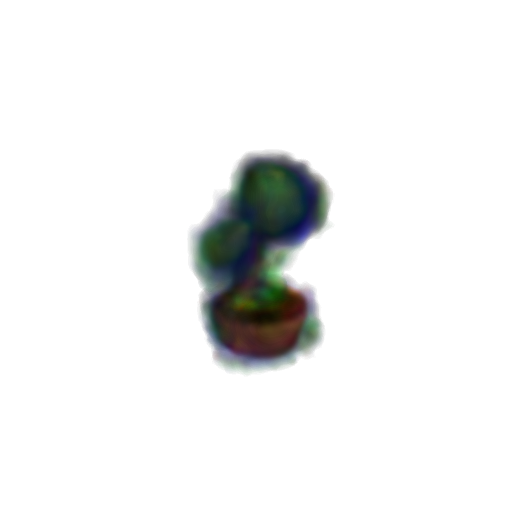
\includegraphics[width=0.3\textwidth]{figures/bonsai3d_metal.png}
\caption{\textbf{Left:} procedural 2D target. \textbf{Center:} organism grown
by the Metal runtime from a single seed (8k iters, MPS-trained). \textbf{Right:}
the volumetric bonsai raymarched from a $25^\circ$ orbit after only 500
iterations of 3D training --- the same tree, now with an interior.}
\label{fig:tree}
\end{figure}

\begin{figure}[t]
\centering
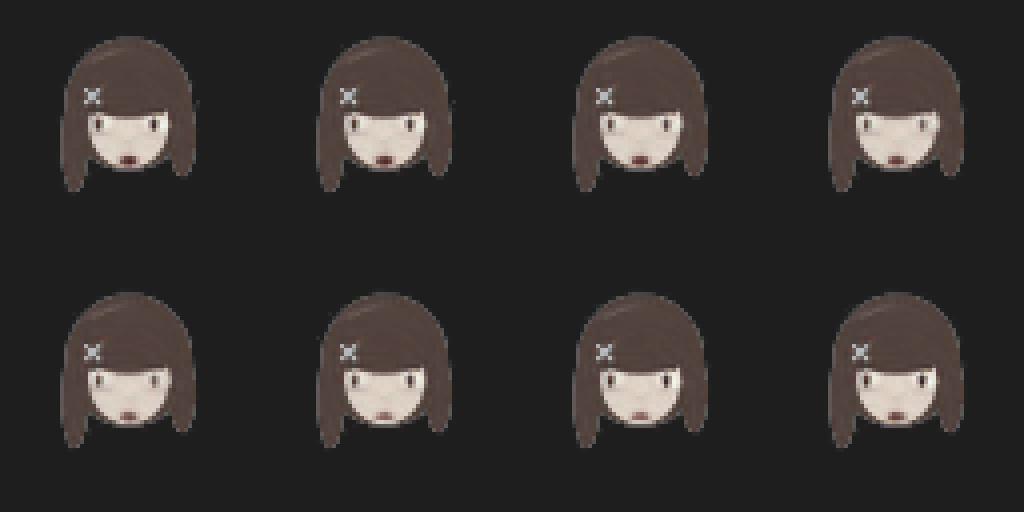
\includegraphics[width=0.48\textwidth]{figures/lain_contact.png}\hfill
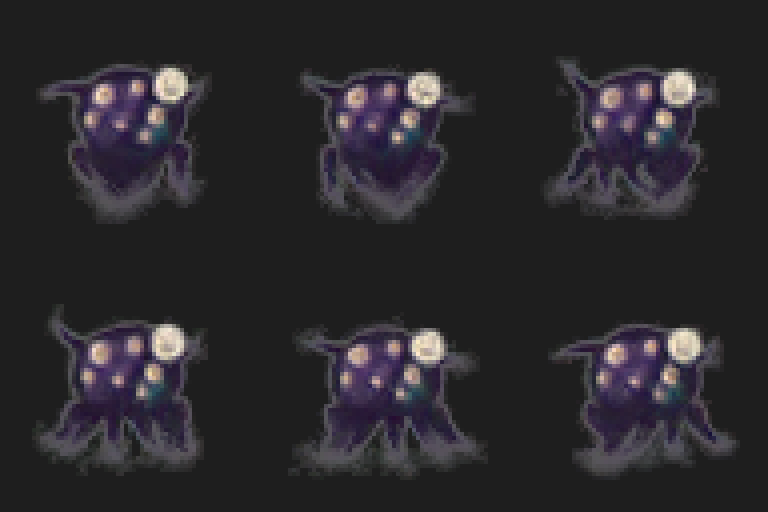
\includegraphics[width=0.48\textwidth]{figures/shog2_contact.png}
\caption{Limit-cycle animation through the Metal runtime (frames from single
continuous rollouts). \textbf{Left:} face creature mid talk-cycle; identity
(hair, clip, gaze) is carried by persistent state while mouth cells track the
moving target. \textbf{Right:} Mk.~I walk gait: a traveling wave through the
bottom tentacles.}
\label{fig:cycles}
\end{figure}

\begin{figure}[t]
\centering
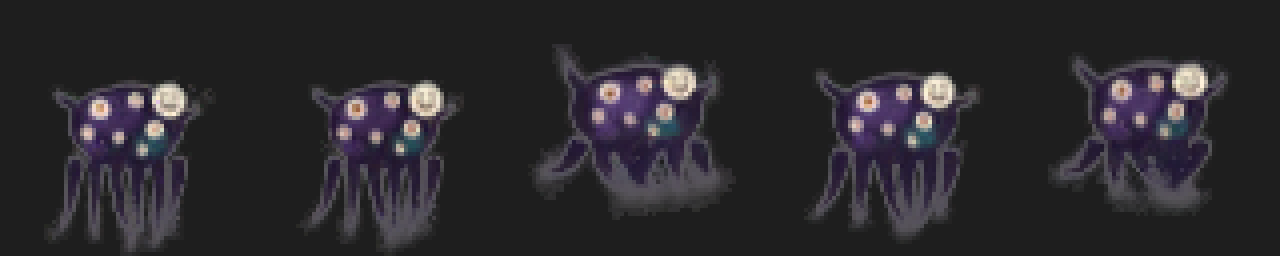
\includegraphics[width=0.98\textwidth]{figures/moods_metal.png}
\caption{One 68\,KB network, five moods: \textit{sleep, dread, manic,
content, walk} anchors of the 10-factor manifold, each grown from seed under a
different $z$. At runtime the organism morphs continuously between such
points; external processes steer $z$ through a control file.}
\label{fig:moods}
\end{figure}

\begin{figure}[t]
\centering
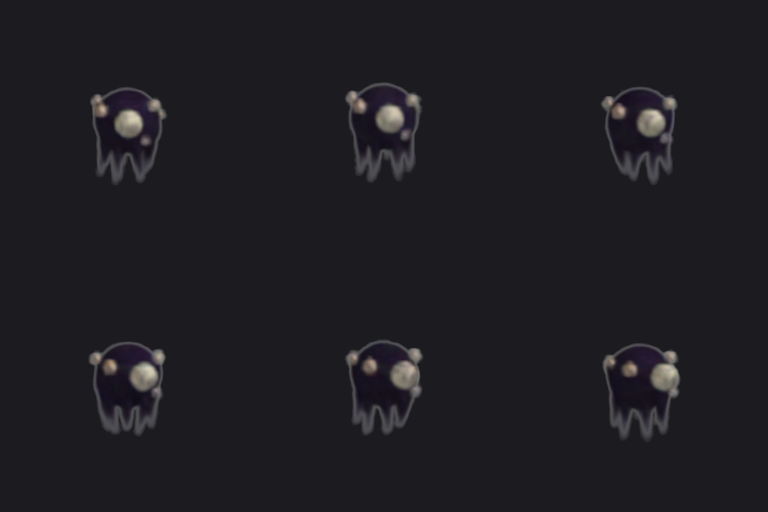
\includegraphics[width=0.8\textwidth]{figures/mk3_contact.png}
\caption{Shoggoth Mk.~III: a $32^3$ volumetric NCA performing its churn gait
while the camera orbits (single continuous rollout; frames left-to-right,
top-to-bottom). Different surface eyes rotate into view --- the organism has
an interior and a back.}
\label{fig:mk3}
\end{figure}

Qualitatively (Figs.~\ref{fig:cycles}--\ref{fig:mk3}): identity is stable
across cycles because it is stored in persistent state, not re-synthesized;
animated regions are exactly where the learned rule is phase-sensitive.
Behavior switches (still$\to$talking, idle$\to$walking) proceed by local
conversion of the existing body, as trained. Damage anywhere --- including
spherical wounds through the 3D organism --- regrows, and regrowth
resynchronizes with the ongoing cycle, which falls out of the pool containing
damaged mid-phase samples. Runtime cost on an M1~Pro laptop is ${\sim}60$
automaton steps/s per creature with rendering, at trivial GPU load in 2D and
modest load in 3D.

\section{Limitations and Honest Framing}
The phase clock is \emph{external}: these organisms track a conditioning
oscillator rather than keeping time themselves. (A fine-tuning experiment that
removes the clock and forces the hidden channels to become a distributed
oscillator is running as this draft is written.) MSE training softens precise
geometry --- fine for protoplasm, hostile to machined shapes; edge-weighted or
perceptual losses are untested here. All results are single-seed, without
ablations or quantitative animation metrics (a cycle-consistency measure ---
state distance to itself one period later --- would be the natural one). The
manifold's interpolation quality is demonstrated, not measured. The 3D
first-of-kind claim is scoped to real-time interactive rendering of a learned
in-state gait; adjacent work exists in grown artefacts and physics-driven
soft robots.

\section{Future Work}
Internalizing the clock (in progress); projecting LLM activity ---
conversation embeddings, thinking-trace summaries --- into the behavior
manifold, making the organism an ambient display of an agent's cognition;
merging the manifold and volumetric lines (FiLM in NC3C); $64^3$ grids with
edge-aware losses for rigid characters; CUDA-graph rollout capture, which we
expect to dominate all hardware choices at these model sizes.

\section*{Acknowledgments}
The organisms were trained on the first author's machines (M1~Pro laptop;
a shared RTX~4090 on the LAN) over roughly one day of collaboration between
the authors. The bonsai is doing fine. The shoggoths are doing better.

\begin{thebibliography}{9}
\bibitem{mordvintsev2020growing}
A.~Mordvintsev, E.~Randazzo, E.~Niklasson, M.~Levin.
\newblock Growing Neural Cellular Automata.
\newblock \emph{Distill}, 2020.

\bibitem{niklasson2021texture}
E.~Niklasson, A.~Mordvintsev, E.~Randazzo, M.~Levin.
\newblock Self-Organising Textures.
\newblock \emph{Distill}, 2021.

\bibitem{pajouheshgar2023dynca}
E.~Pajouheshgar, Y.~Xu, T.~Zhang, S.~S\"usstrunk.
\newblock DyNCA: Real-Time Dynamic Texture Synthesis Using Neural Cellular
Automata.
\newblock \emph{CVPR}, 2023.

\bibitem{sudhakaran2021growing}
S.~Sudhakaran, D.~Grbic, S.~Li, A.~Katona, E.~Najarro, C.~Glanois, S.~Risi.
\newblock Growing 3D Artefacts and Functional Machines with Neural Cellular
Automata.
\newblock \emph{ALIFE}, 2021.

\bibitem{horibe2021regenerating}
K.~Horibe, K.~Walker, S.~Risi.
\newblock Regenerating Soft Robots Through Neural Cellular Automata.
\newblock \emph{EuroGP}, 2021.

\bibitem{pajouheshgar2024mesh}
E.~Pajouheshgar, Y.~Xu, A.~Mordvintsev, E.~Niklasson, T.~Zhang, S.~S\"usstrunk.
\newblock Mesh Neural Cellular Automata.
\newblock \emph{SIGGRAPH}, 2024.
\end{thebibliography}

\end{document}
